\section{Results}
\label{sec:4}

% \subsection{Generated dataset}
\label{sec:4.1}

The main dataset was generated with Isomorph-Reborn using the ISOMORPH network at a strain level of 75, in the flow representation (hence without inventory effects). Severity ranges from 0.68 to 1, disruption duration from 8 to 24 days, and the strain rate from 1.08 to 1.42. The critical thresholds of the profiles were raised to 0.98, 0.95, and 0.92. With a median minimum service level close to 0.87, the nominal thresholds left the prudent and delayed profiles almost always inactive. The ranking of the profiles, the sole object of the comparison, remains the same.

The dataset used contains the 2,000 scenarios, that is, 8,000 crisis versions, split roughly equally among the five disruption types. The curve fit is satisfactory, with a median coefficient of determination of 0.88. The cumulative loss IPC tracks the service actually lost very closely (correlation of 0.97). This is why it serves as the main indicator in what follows (\voirSM{S6.1}).

\subsection{Effect of management policies}
\label{sec:4.2}

Table~\ref{tab:d12} compares the four policies over the 2,000 crises. The reactive profile clearly comes out ahead. It reduces the cumulative loss by a median 82\% relative to no reaction, against 17\% for the prudent profile and 0\% for the delayed profile, which does not act in half of the crises. All three differences are significant (paired Wilcoxon signed-rank test, $p < 10^{-150}$). Since levers have no cost in the model, acting early never has a drawback. This advantage stems in part from the very construction of the model.


\begin{table*}[htbp]
\caption{Reaction and resilience by management policy (2,000 crises).}
\label{tab:d12}
\footnotesize
\begin{tabularx}{\textwidth}{@{}LP{2.3cm}P{2.3cm}P{2.3cm}P{2.3cm}@{}}
\toprule
\textbf{Indicator} & \textbf{No reaction} & \textbf{Reactive} & \textbf{Prudent} & \textbf{Delayed} \\
\toprule
Versions with at least one lever engaged & not applicable & 98\% & 88\% & 56\% \\
\midrule
Mean number of levers engaged & 0 & 2.8 & 2.0 & 0.7 \\
\midrule
Detection, days after onset (median) & not applicable & 0 & 1 & 3 \\
\midrule
Minimum service level (median) & 0.87 & 0.89 & 0.88 & 0.87 \\
\midrule
Days before return to normal (median) & 14 & 4 & 11 & 13 \\
\midrule
IPC, median [quartiles] & 0.67 [0.43; 1.02] & 0.11 [0.07; 0.18] & 0.51 [0.36; 0.69] & 0.58 [0.43; 0.74] \\
\midrule
Share of lost service avoided & reference & 73\% & 18\% & 14\% \\
\bottomrule
\end{tabularx}
\end{table*}

Reacting shortens the crisis without reducing its depth. The minimum service level is almost the same under all policies, but the return to normal occurs on the fourth day under the reactive profile, against the fourteenth day with no reaction (Fig.~\ref{fig:d5}). Under the reactive profile, the cumulative loss no longer depends on the disruption duration (Spearman rank correlation of 0.01), whereas it clearly does with no reaction (0.48). Severity, by contrast, carries little weight (0.08); within this range, it is the persistence of the disruption that makes the crisis.

\begin{center}
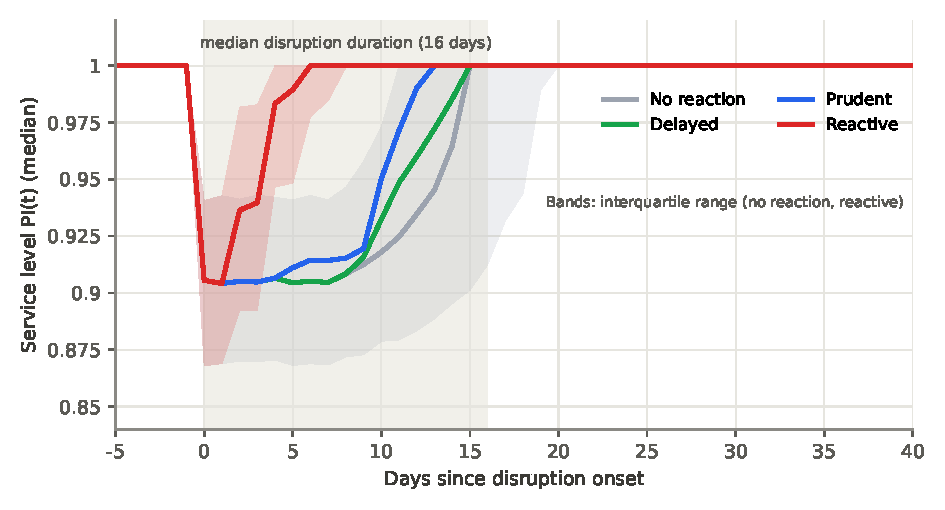
\includegraphics[width=0.5\textwidth]{figures/Fig5_median_trajectory_EN.pdf}
\captionof{figure}{Median service level trajectory by management policy (2,000 crises aligned on disruption onset).}\label{fig:d5}
\end{center}

The effectiveness of a policy varies with the disruption type. The prudent profile, for example, makes no difference to a supplier failure but reduces the loss from a congestion by 41\% (\voirSM{S6.2}). Duration also matters. If the loss is split into three levels of equal size, the prudent profile reaches the same level as the reactive profile in 18\% of the crises, a share that rises to 31\% for disruptions of 12 days or less and falls to 11\% beyond 18 days. A short crisis can therefore be handled with a light response, whereas a long crisis calls for reactivity.

These proportions hold on a second network. On a control batch of 500 scenarios generated on the parametric network, the share of lost service avoided reaches 67\%, 17\%, and 13\% for the reactive, prudent, and delayed profiles. Topology nevertheless changes the effectiveness of the levers. On this network, whose backup routes are narrow, the reactive profile reduces the loss from a link cut by only 25\% and that from a closure by 53\%, against 73\% and 82\% on ISOMORPH.

\subsection{Steering with the Bayesian model}
\label{sec:4.3}

The learned network recovers the mechanism described above on its own. Its structure (Fig.~\ref{fig:d6}) has 41 arcs, none of which runs against the tier order. The cumulative loss depends directly on the policy, the depth $h$, and the duration $d$ of the plateau. This duration in turn depends on the policy, the disruption duration, and the reaction delay.

\begin{center}
\resizebox{\textwidth}{!}{% Figure: Bayesian network learned under constraints, with the marginal distribution of each variable
% (data: .bif file exported by BayesArtist; marginals obtained by exact inference without evidence)
\begin{tikzpicture}[
  bx/.style={draw=#1, fill=#1!10, rounded corners=3pt, minimum width=3.25cm, inner sep=0pt},
  tt/.style={font=\scriptsize\bfseries, text=black!80, anchor=north, align=center, inner sep=1pt},
  ml/.style={font=\tiny, anchor=west, inner sep=0pt},
  pc/.style={font=\tiny, anchor=east, inner sep=0pt},
  a/.style={-{Stealth[length=1.4mm]}, black!30, thin},
  m/.style={-{Stealth[length=2mm]}, polreac, very thick}]
  \node[font=\small\bfseries, text=black!70] at (0.00,6.56) {Context};
  % cible
  \node[bx=palctx, minimum height=1.360cm] (cible) at (0.00,3.945) {};
  \node[tt] at (0.00,4.585) {Target position};
  \node[ml] at (-1.53,4.060) {Bottleneck};
  \fill[black!8] (0.095,3.975) rectangle (0.815,4.145);
  \fill[palctx] (0.095,3.975) rectangle (0.137,4.145);
  \node[pc] at (1.54,4.060) {5.8\,\%};
  \node[ml] at (-1.53,3.770) {Redund. site};
  \fill[black!8] (0.095,3.685) rectangle (0.815,3.855);
  \fill[palctx] (0.095,3.685) rectangle (0.488,3.855);
  \node[pc] at (1.54,3.770) {54.6\,\%};
  \node[ml] at (-1.53,3.480) {Whole netw.};
  \fill[black!8] (0.095,3.395) rectangle (0.815,3.565);
  \fill[palctx] (0.095,3.395) rectangle (0.380,3.565);
  \node[pc] at (1.54,3.480) {39.6\,\%};
  % partcrit
  \node[bx=palctx, minimum height=1.630cm] (partcrit) at (0.00,2.050) {};
  \node[tt] at (0.00,2.825) {Share of critical\\items};
  \node[ml] at (-1.53,2.030) {Low};
  \fill[black!8] (0.095,1.945) rectangle (0.815,2.115);
  \fill[palctx] (0.095,1.945) rectangle (0.335,2.115);
  \node[pc] at (1.54,2.030) {33.4\,\%};
  \node[ml] at (-1.53,1.740) {Medium};
  \fill[black!8] (0.095,1.655) rectangle (0.815,1.825);
  \fill[palctx] (0.095,1.655) rectangle (0.335,1.825);
  \node[pc] at (1.54,1.740) {33.4\,\%};
  \node[ml] at (-1.53,1.450) {High};
  \fill[black!8] (0.095,1.365) rectangle (0.815,1.535);
  \fill[palctx] (0.095,1.365) rectangle (0.334,1.535);
  \node[pc] at (1.54,1.450) {33.2\,\%};
  % nature
  \node[bx=palctx, minimum height=1.940cm] (nature) at (0.00,-0.135) {};
  \node[tt] at (0.00,0.795) {Nature};
  \node[ml] at (-1.53,0.270) {Supplier fail.};
  \fill[black!8] (0.095,0.185) rectangle (0.815,0.355);
  \fill[palctx] (0.095,0.185) rectangle (0.250,0.355);
  \node[pc] at (1.54,0.270) {21.5\,\%};
  \node[ml] at (-1.53,-0.020) {Link cut};
  \fill[black!8] (0.095,-0.105) rectangle (0.815,0.065);
  \fill[palctx] (0.095,-0.105) rectangle (0.233,0.065);
  \node[pc] at (1.54,-0.020) {19.1\,\%};
  \node[ml] at (-1.53,-0.310) {Site closure};
  \fill[black!8] (0.095,-0.395) rectangle (0.815,-0.225);
  \fill[palctx] (0.095,-0.395) rectangle (0.238,-0.225);
  \node[pc] at (1.54,-0.310) {19.8\,\%};
  \node[ml] at (-1.53,-0.600) {Demand surge};
  \fill[black!8] (0.095,-0.685) rectangle (0.815,-0.515);
  \fill[palctx] (0.095,-0.685) rectangle (0.241,-0.515);
  \node[pc] at (1.54,-0.600) {20.3\,\%};
  \node[ml] at (-1.53,-0.890) {Congestion};
  \fill[black!8] (0.095,-0.975) rectangle (0.815,-0.805);
  \fill[palctx] (0.095,-0.975) rectangle (0.235,-0.805);
  \node[pc] at (1.54,-0.890) {19.4\,\%};
  % severite
  \node[bx=palctx, minimum height=1.360cm] (severite) at (0.00,-2.185) {};
  \node[tt] at (0.00,-1.545) {Severity};
  \node[ml] at (-1.53,-2.070) {Low};
  \fill[black!8] (0.095,-2.155) rectangle (0.815,-1.985);
  \fill[palctx] (0.095,-2.155) rectangle (0.335,-1.985);
  \node[pc] at (1.54,-2.070) {33.4\,\%};
  \node[ml] at (-1.53,-2.360) {Medium};
  \fill[black!8] (0.095,-2.445) rectangle (0.815,-2.275);
  \fill[palctx] (0.095,-2.445) rectangle (0.335,-2.275);
  \node[pc] at (1.54,-2.360) {33.4\,\%};
  \node[ml] at (-1.53,-2.650) {High};
  \fill[black!8] (0.095,-2.735) rectangle (0.815,-2.565);
  \fill[palctx] (0.095,-2.735) rectangle (0.334,-2.565);
  \node[pc] at (1.54,-2.650) {33.2\,\%};
  % duree
  \node[bx=palctx, minimum height=1.360cm] (duree) at (0.00,-3.945) {};
  \node[tt] at (0.00,-3.305) {Duration};
  \node[ml] at (-1.53,-3.830) {Low};
  \fill[black!8] (0.095,-3.915) rectangle (0.815,-3.745);
  \fill[palctx] (0.095,-3.915) rectangle (0.346,-3.745);
  \node[pc] at (1.54,-3.830) {34.8\,\%};
  \node[ml] at (-1.53,-4.120) {Medium};
  \fill[black!8] (0.095,-4.205) rectangle (0.815,-4.035);
  \fill[palctx] (0.095,-4.205) rectangle (0.328,-4.035);
  \node[pc] at (1.54,-4.120) {32.3\,\%};
  \node[ml] at (-1.53,-4.410) {High};
  \fill[black!8] (0.095,-4.495) rectangle (0.815,-4.325);
  \fill[palctx] (0.095,-4.495) rectangle (0.332,-4.325);
  \node[pc] at (1.54,-4.410) {32.9\,\%};
  \node[font=\small\bfseries, text=black!70] at (4.00,6.56) {Policy};
  % profil
  \node[bx=palpol, minimum height=1.650cm] (profil) at (4.00,0.000) {};
  \node[tt] at (4.00,0.785) {Management policy};
  \node[ml] at (2.46,0.260) {No reaction};
  \fill[black!8] (4.095,0.175) rectangle (4.815,0.345);
  \fill[palpol] (4.095,0.175) rectangle (4.275,0.345);
  \node[pc] at (5.54,0.260) {25.0\,\%};
  \node[ml] at (2.46,-0.030) {Reactive};
  \fill[black!8] (4.095,-0.115) rectangle (4.815,0.055);
  \fill[palpol] (4.095,-0.115) rectangle (4.275,0.055);
  \node[pc] at (5.54,-0.030) {25.0\,\%};
  \node[ml] at (2.46,-0.320) {Prudent};
  \fill[black!8] (4.095,-0.405) rectangle (4.815,-0.235);
  \fill[palpol] (4.095,-0.405) rectangle (4.275,-0.235);
  \node[pc] at (5.54,-0.320) {25.0\,\%};
  \node[ml] at (2.46,-0.610) {Delayed};
  \fill[black!8] (4.095,-0.695) rectangle (4.815,-0.525);
  \fill[palpol] (4.095,-0.695) rectangle (4.275,-0.525);
  \node[pc] at (5.54,-0.610) {25.0\,\%};
  \node[font=\small\bfseries, text=black!70] at (8.00,6.56) {Response};
  % detection
  \node[bx=palrep, minimum height=1.940cm] (detection) at (8.00,4.990) {};
  \node[tt] at (8.00,5.920) {Detection};
  \node[ml] at (6.46,5.395) {D0};
  \fill[black!8] (8.095,5.310) rectangle (8.815,5.480);
  \fill[palrep] (8.095,5.310) rectangle (8.262,5.480);
  \node[pc] at (9.54,5.395) {23.2\,\%};
  \node[ml] at (6.46,5.105) {D1-D2};
  \fill[black!8] (8.095,5.020) rectangle (8.815,5.190);
  \fill[palrep] (8.095,5.020) rectangle (8.243,5.190);
  \node[pc] at (9.54,5.105) {20.6\,\%};
  \node[ml] at (6.46,4.815) {D3+};
  \fill[black!8] (8.095,4.730) rectangle (8.815,4.900);
  \fill[palrep] (8.095,4.730) rectangle (8.216,4.900);
  \node[pc] at (9.54,4.815) {16.8\,\%};
  \node[ml] at (6.46,4.525) {Not detected};
  \fill[black!8] (8.095,4.440) rectangle (8.815,4.610);
  \fill[palrep] (8.095,4.440) rectangle (8.199,4.610);
  \node[pc] at (9.54,4.525) {14.4\,\%};
  \node[ml] at (6.46,4.235) {n/a};
  \fill[black!8] (8.095,4.150) rectangle (8.815,4.320);
  \fill[palrep] (8.095,4.150) rectangle (8.275,4.320);
  \node[pc] at (9.54,4.235) {25.0\,\%};
  % nbleviers
  \node[bx=palrep, minimum height=1.650cm] (nbleviers) at (8.00,2.795) {};
  \node[tt] at (8.00,3.580) {Number of levers};
  \node[ml] at (6.46,3.055) {0};
  \fill[black!8] (8.095,2.970) rectangle (8.815,3.140);
  \fill[palrep] (8.095,2.970) rectangle (8.377,3.140);
  \node[pc] at (9.54,3.055) {39.2\,\%};
  \node[ml] at (6.46,2.765) {1};
  \fill[black!8] (8.095,2.680) rectangle (8.815,2.850);
  \fill[palrep] (8.095,2.680) rectangle (8.213,2.850);
  \node[pc] at (9.54,2.765) {16.4\,\%};
  \node[ml] at (6.46,2.475) {2};
  \fill[black!8] (8.095,2.390) rectangle (8.815,2.560);
  \fill[palrep] (8.095,2.390) rectangle (8.263,2.560);
  \node[pc] at (9.54,2.475) {23.3\,\%};
  \node[ml] at (6.46,2.185) {3+};
  \fill[black!8] (8.095,2.100) rectangle (8.815,2.270);
  \fill[palrep] (8.095,2.100) rectangle (8.248,2.270);
  \node[pc] at (9.54,2.185) {21.2\,\%};
  % lag
  \node[bx=palrep, minimum height=1.650cm] (lag) at (8.00,0.745) {};
  \node[tt] at (8.00,1.530) {Reaction delay};
  \node[ml] at (6.46,1.005) {Short};
  \fill[black!8] (8.095,0.920) rectangle (8.815,1.090);
  \fill[palrep] (8.095,0.920) rectangle (8.257,1.090);
  \node[pc] at (9.54,1.005) {22.5\,\%};
  \node[ml] at (6.46,0.715) {Medium};
  \fill[black!8] (8.095,0.630) rectangle (8.815,0.800);
  \fill[palrep] (8.095,0.630) rectangle (8.278,0.800);
  \node[pc] at (9.54,0.715) {25.4\,\%};
  \node[ml] at (6.46,0.425) {Long};
  \fill[black!8] (8.095,0.340) rectangle (8.815,0.510);
  \fill[palrep] (8.095,0.340) rectangle (8.187,0.510);
  \node[pc] at (9.54,0.425) {12.8\,\%};
  \node[ml] at (6.46,0.135) {n/a};
  \fill[black!8] (8.095,0.050) rectangle (8.815,0.220);
  \fill[palrep] (8.095,0.050) rectangle (8.377,0.220);
  \node[pc] at (9.54,0.135) {39.2\,\%};
  % fstock
  \node[bx=palrep, minimum height=1.070cm] (fstock) at (8.00,-1.015) {};
  \node[tt] at (8.00,-0.520) {Inventory levers};
  \node[ml] at (6.46,-1.045) {No};
  \fill[black!8] (8.095,-1.130) rectangle (8.815,-0.960);
  \fill[palrep] (8.095,-1.130) rectangle (8.641,-0.960);
  \node[pc] at (9.54,-1.045) {75.8\,\%};
  \node[ml] at (6.46,-1.335) {Yes};
  \fill[black!8] (8.095,-1.420) rectangle (8.815,-1.250);
  \fill[palrep] (8.095,-1.420) rectangle (8.269,-1.250);
  \node[pc] at (9.54,-1.335) {24.2\,\%};
  % freroutage
  \node[bx=palrep, minimum height=1.070cm] (freroutage) at (8.00,-2.485) {};
  \node[tt] at (8.00,-1.990) {Rerouting levers};
  \node[ml] at (6.46,-2.515) {No};
  \fill[black!8] (8.095,-2.600) rectangle (8.815,-2.430);
  \fill[palrep] (8.095,-2.600) rectangle (8.650,-2.430);
  \node[pc] at (9.54,-2.515) {77.1\,\%};
  \node[ml] at (6.46,-2.805) {Yes};
  \fill[black!8] (8.095,-2.890) rectangle (8.815,-2.720);
  \fill[palrep] (8.095,-2.890) rectangle (8.260,-2.720);
  \node[pc] at (9.54,-2.805) {22.9\,\%};
  % fcapacite
  \node[bx=palrep, minimum height=1.070cm] (fcapacite) at (8.00,-3.955) {};
  \node[tt] at (8.00,-3.460) {Capacity levers};
  \node[ml] at (6.46,-3.985) {No};
  \fill[black!8] (8.095,-4.070) rectangle (8.815,-3.900);
  \fill[palrep] (8.095,-4.070) rectangle (8.586,-3.900);
  \node[pc] at (9.54,-3.985) {68.2\,\%};
  \node[ml] at (6.46,-4.275) {Yes};
  \fill[black!8] (8.095,-4.360) rectangle (8.815,-4.190);
  \fill[palrep] (8.095,-4.360) rectangle (8.324,-4.190);
  \node[pc] at (9.54,-4.275) {31.8\,\%};
  % fdemande
  \node[bx=palrep, minimum height=1.070cm] (fdemande) at (8.00,-5.425) {};
  \node[tt] at (8.00,-4.930) {Demand levers};
  \node[ml] at (6.46,-5.455) {No};
  \fill[black!8] (8.095,-5.540) rectangle (8.815,-5.370);
  \fill[palrep] (8.095,-5.540) rectangle (8.628,-5.370);
  \node[pc] at (9.54,-5.455) {74.0\,\%};
  \node[ml] at (6.46,-5.745) {Yes};
  \fill[black!8] (8.095,-5.830) rectangle (8.815,-5.660);
  \fill[palrep] (8.095,-5.830) rectangle (8.282,-5.660);
  \node[pc] at (9.54,-5.745) {26.0\,\%};
  \node[font=\small\bfseries, text=black!70] at (12.00,6.56) {Mechanism};
  % beta
  \node[bx=palmec, minimum height=1.360cm] (beta) at (12.00,2.640) {};
  \node[tt] at (12.00,3.280) {$\beta$ (recovery)};
  \node[ml] at (10.46,2.755) {Low};
  \fill[black!8] (12.095,2.670) rectangle (12.815,2.840);
  \fill[palmec] (12.095,2.670) rectangle (12.337,2.840);
  \node[pc] at (13.54,2.755) {33.6\,\%};
  \node[ml] at (10.46,2.465) {Medium};
  \fill[black!8] (12.095,2.380) rectangle (12.815,2.550);
  \fill[palmec] (12.095,2.380) rectangle (12.331,2.550);
  \node[pc] at (13.54,2.465) {32.8\,\%};
  \node[ml] at (10.46,2.175) {High};
  \fill[black!8] (12.095,2.090) rectangle (12.815,2.260);
  \fill[palmec] (12.095,2.090) rectangle (12.337,2.260);
  \node[pc] at (13.54,2.175) {33.6\,\%};
  % h
  \node[bx=palmec, minimum height=1.360cm] (h) at (12.00,0.880) {};
  \node[tt] at (12.00,1.520) {$h$ (depth)};
  \node[ml] at (10.46,0.995) {Low};
  \fill[black!8] (12.095,0.910) rectangle (12.815,1.080);
  \fill[palmec] (12.095,0.910) rectangle (12.338,1.080);
  \node[pc] at (13.54,0.995) {33.7\,\%};
  \node[ml] at (10.46,0.705) {Medium};
  \fill[black!8] (12.095,0.620) rectangle (12.815,0.790);
  \fill[palmec] (12.095,0.620) rectangle (12.335,0.790);
  \node[pc] at (13.54,0.705) {33.4\,\%};
  \node[ml] at (10.46,0.415) {High};
  \fill[black!8] (12.095,0.330) rectangle (12.815,0.500);
  \fill[palmec] (12.095,0.330) rectangle (12.331,0.500);
  \node[pc] at (13.54,0.415) {32.8\,\%};
  % alpha
  \node[bx=palmec, minimum height=1.360cm] (alpha) at (12.00,-0.880) {};
  \node[tt] at (12.00,-0.240) {$\alpha$ (drop)};
  \node[ml] at (10.46,-0.765) {Low};
  \fill[black!8] (12.095,-0.850) rectangle (12.815,-0.680);
  \fill[palmec] (12.095,-0.850) rectangle (12.334,-0.680);
  \node[pc] at (13.54,-0.765) {33.2\,\%};
  \node[ml] at (10.46,-1.055) {Medium};
  \fill[black!8] (12.095,-1.140) rectangle (12.815,-0.970);
  \fill[palmec] (12.095,-1.140) rectangle (12.335,-0.970);
  \node[pc] at (13.54,-1.055) {33.3\,\%};
  \node[ml] at (10.46,-1.345) {High};
  \fill[black!8] (12.095,-1.430) rectangle (12.815,-1.260);
  \fill[palmec] (12.095,-1.430) rectangle (12.335,-1.260);
  \node[pc] at (13.54,-1.345) {33.4\,\%};
  % d
  \node[bx=palmec, minimum height=1.360cm] (d) at (12.00,-2.640) {};
  \node[tt] at (12.00,-2.000) {$d$ (plateau duration)};
  \node[ml] at (10.46,-2.525) {Low};
  \fill[black!8] (12.095,-2.610) rectangle (12.815,-2.440);
  \fill[palmec] (12.095,-2.610) rectangle (12.338,-2.440);
  \node[pc] at (13.54,-2.525) {33.8\,\%};
  \node[ml] at (10.46,-2.815) {Medium};
  \fill[black!8] (12.095,-2.900) rectangle (12.815,-2.730);
  \fill[palmec] (12.095,-2.900) rectangle (12.334,-2.730);
  \node[pc] at (13.54,-2.815) {33.2\,\%};
  \node[ml] at (10.46,-3.105) {High};
  \fill[black!8] (12.095,-3.190) rectangle (12.815,-3.020);
  \fill[palmec] (12.095,-3.190) rectangle (12.333,-3.020);
  \node[pc] at (13.54,-3.105) {33.0\,\%};
  \node[font=\small\bfseries, text=black!70] at (16.00,6.56) {Resilience};
  % CRD
  \node[bx=palres, minimum height=1.360cm] (CRD) at (16.00,1.760) {};
  \node[tt] at (16.00,2.400) {CRD};
  \node[ml] at (14.46,1.875) {Low};
  \fill[black!8] (16.095,1.790) rectangle (16.815,1.960);
  \fill[palres] (16.095,1.790) rectangle (16.345,1.960);
  \node[pc] at (17.55,1.875) {34.7\,\%};
  \node[ml] at (14.46,1.585) {Medium};
  \fill[black!8] (16.095,1.500) rectangle (16.815,1.670);
  \fill[palres] (16.095,1.500) rectangle (16.320,1.670);
  \node[pc] at (17.55,1.585) {31.3\,\%};
  \node[ml] at (14.46,1.295) {High};
  \fill[black!8] (16.095,1.210) rectangle (16.815,1.380);
  \fill[palres] (16.095,1.210) rectangle (16.340,1.380);
  \node[pc] at (17.55,1.295) {34.0\,\%};
  % IPC
  \node[bx=palres, minimum height=1.360cm] (IPC) at (16.00,0.000) {};
  \node[tt] at (16.00,0.640) {IPC};
  \node[ml] at (14.46,0.115) {Low};
  \fill[black!8] (16.095,0.030) rectangle (16.815,0.200);
  \fill[palres] (16.095,0.030) rectangle (16.341,0.200);
  \node[pc] at (17.55,0.115) {34.1\,\%};
  \node[ml] at (14.46,-0.175) {Medium};
  \fill[black!8] (16.095,-0.260) rectangle (16.815,-0.090);
  \fill[palres] (16.095,-0.260) rectangle (16.333,-0.090);
  \node[pc] at (17.55,-0.175) {33.0\,\%};
  \node[ml] at (14.46,-0.465) {High};
  \fill[black!8] (16.095,-0.550) rectangle (16.815,-0.380);
  \fill[palres] (16.095,-0.550) rectangle (16.332,-0.380);
  \node[pc] at (17.55,-0.465) {32.9\,\%};
  % TRP
  \node[bx=palres, minimum height=1.360cm] (TRP) at (16.00,-1.760) {};
  \node[tt] at (16.00,-1.120) {TRP};
  \node[ml] at (14.46,-1.645) {Low};
  \fill[black!8] (16.095,-1.730) rectangle (16.815,-1.560);
  \fill[palres] (16.095,-1.730) rectangle (16.335,-1.560);
  \node[pc] at (17.55,-1.645) {33.3\,\%};
  \node[ml] at (14.46,-1.935) {Medium};
  \fill[black!8] (16.095,-2.020) rectangle (16.815,-1.850);
  \fill[palres] (16.095,-2.020) rectangle (16.344,-1.850);
  \node[pc] at (17.55,-1.935) {34.6\,\%};
  \node[ml] at (14.46,-2.225) {High};
  \fill[black!8] (16.095,-2.310) rectangle (16.815,-2.140);
  \fill[palres] (16.095,-2.310) rectangle (16.326,-2.140);
  \node[pc] at (17.55,-2.225) {32.1\,\%};
  \begin{scope}[on background layer]
    \draw[a] (cible.west) to[bend right=26] (nature.west);
    \draw[a] (cible.east) -- (detection.west);
    \draw[a] (profil.east) -- (detection.west);
    \draw[a] (nature.west) to[bend right=26] (severite.west);
    \draw[a] (nature.east) -- (nbleviers.west);
    \draw[a] (detection.east) to[bend left=26] (nbleviers.east);
    \draw[a] (severite.west) to[bend right=26] (duree.west);
    \draw[a] (profil.east) -- (beta.west);
    \draw[a] (nbleviers.east) -- (beta.west);
    \draw[a] (nature.east) -- (freroutage.west);
    \draw[a] (profil.east) -- (freroutage.west);
    \draw[a] (nbleviers.east) to[bend left=26] (freroutage.east);
    \draw[a] (nature.east) -- (fdemande.west);
    \draw[a] (profil.east) -- (fdemande.west);
    \draw[a] (nbleviers.east) to[bend left=26] (fdemande.east);
    \draw[a] (beta.east) to[bend left=26] (h.east);
    \draw[a] (detection.east) -- (h.west);
    \draw[a] (fdemande.east) -- (h.west);
    \draw[a] (profil.east) -- (fstock.west);
    \draw[a] (nbleviers.east) to[bend left=26] (fstock.east);
    \draw[a] (freroutage.east) to[bend right=26] (fstock.east);
    \draw[a] (h.east) to[bend left=26] (alpha.east);
    \draw[a] (beta.east) to[bend left=26] (alpha.east);
    \draw[a] (detection.east) to[bend left=26] (lag.east);
    \draw[a] (nbleviers.east) to[bend left=26] (lag.east);
    \draw[a] (fstock.east) to[bend right=26] (lag.east);
    \draw[a] (nature.east) -- (fcapacite.west);
    \draw[a] (nbleviers.east) to[bend left=26] (fcapacite.east);
    \draw[a] (fstock.east) to[bend left=26] (fcapacite.east);
    \draw[m] (profil.east) -- (d.west);
    \draw[m] (duree.east) -- (d.west);
    \draw[m] (lag.east) -- (d.west);
    \draw[m] (profil.east) -- (IPC.west);
    \draw[m] (h.east) -- (IPC.west);
    \draw[m] (d.east) -- (IPC.west);
    \draw[a] (d.east) -- (CRD.west);
    \draw[a] (alpha.east) -- (CRD.west);
    \draw[a] (beta.east) -- (CRD.west);
    \draw[a] (duree.east) -- (TRP.west);
    \draw[a] (d.east) -- (TRP.west);
    \draw[a] (CRD.east) to[bend left=26] (TRP.east);
  \end{scope}
  \node[font=\scriptsize, text=black!65, anchor=north, text width=17cm, align=center] at (8.00,-6.21) {Thick line: main path (the policy acts on the duration $d$ of the degraded plateau, which determines the cumulative loss IPC). 20 variables, 41 arcs. Bars: marginal probability of each state.};
\end{tikzpicture}
}
\captionof{figure}{Bayesian network learned under constraints, with variables colored by tier of the temporal order of a crisis; each node gives the marginal probability of its states.}\label{fig:d6}
\end{center}

Using only the variables known at decision time, the prognosis correctly classifies 65\% of the test crises, against 60\% for a model that knows only the management policy applied (no reaction, reactive, prudent, or delayed) and 34\% for an uninformed model, which assigns each class its frequency and selects the most frequent one. The corresponding Brier scores are 0.466, 0.494, and 0.667. The learning curve is almost flat, which indicates that accuracy is limited by the information available at decision time rather than by the size of the dataset. The diagnosis is well calibrated for policy and duration. For the high-loss test crises, the posterior probabilities of the policies reproduce their observed frequencies to within 0.01.

The recommendation that can be made depends on the objective. If the aim is a low loss, only the reactive profile succeeds consistently and the rule always recommends it. If the aim is only to avoid a high loss, a trade-off appears between safety and restraint, governed by the threshold $\theta$ (Table~\ref{tab:d15}).

\begin{table*}[htbp]
\caption{Recommendation on the test crises, with the objective of a cumulative loss that is not high.}
\label{tab:d15}
\footnotesize
\begin{tabularx}{\textwidth}{@{}LLL@{}}
\toprule
\textbf{Rule} & \textbf{Objective met} & \textbf{Recommendations lighter than the reactive profile} \\
\midrule
Always the reactive profile & 99.2\% & 0\% \\
Learned network, $\theta$ = 0.9 & 99.2\% & 0\% \\
Learned network, $\theta$ = 0.8 & 97.5\% & 15\% \\
Learned network, $\theta$ = 0.7 & 86.2\% & 37\% \\
Learned network, $\theta$ = 0.6 & 69.5\% & 84\% \\
A posteriori reference: lightest successful policy & 99.2\% & 67\% \\
\bottomrule
\end{tabularx}
\end{table*}

With $\theta$ = 0.8, that is, selecting the least interventionist policy among those that meet the objective with a probability of at least 0.8, the network recommends a lighter policy in about one crisis out of seven. The objective is met in 97.5\% of cases, less than two points below the most interventionist policy. This restraint rests entirely on the forecast duration of the disruption. If this information is removed from the crisis description, the rule no longer recommends any lighter policy. Knowing the probable duration of a disruption therefore has decision value in itself. For the short closure of a redundant site, for example, the prudent profile meets the objective with a probability of 0.80 and becomes the recommendation, whereas for the long closure of a bottleneck, only the reactive profile does so (\voirSM{S6.3}).

Figure~\ref{fig:carte} extends this analysis to the seven contexts allowed by the ISOMORPH topology, by backward inference and for the objective of a low loss. The reactive profile is the most probable everywhere, and all the more so as the disruption lasts longer, its posterior probability rising from 0.51--0.58 for a short disruption to 0.72--0.79 for a long one. For a short disruption, each of the other policies keeps a probability between 0.12 and 0.18, a sign that a low loss then remains attainable without a rapid reaction.

\begin{center}
\begin{minipage}{\textwidth}\centering
% Figure: recommendation map by backward inference on the learned network, as a scatter plot.
% Posterior probability of each profile given IPC = low, for the seven contexts (nature, target position),
% one panel per disruption duration. Green: most probable policy of the context; red: other policies.
% Values identical to the former map (exact inference on the learned network, .bif file).
\begin{tikzpicture}
\pgfplotsset{carte/.style={width=5.6cm, height=5.6cm, xmin=0.5, xmax=4.5, ymin=0, ymax=0.85,
  xtick={1,2,3,4}, xticklabels={None,Delayed,Prudent,Reactive},
  ytick={0,0.2,0.4,0.6,0.8}, yticklabel style={/pgf/number format/.cd,fixed,fixed zerofill,precision=1,use period},
  tick label style={font=\scriptsize}, xticklabel style={font=\fontsize{6}{7}\selectfont}, label style={font=\scriptsize}, title style={font=\small\bfseries},
  ymajorgrids, grid style={gray!20}, axis lines*=left, clip=false}}
\begin{axis}[carte, title={Short duration}, at={(0.0cm,0)}, ylabel={Posterior probability of the profile}]
  \addplot[only marks, mark=*, mark size=1.8pt, appreac, fill opacity=0.75, draw opacity=0.9] coordinates {(0.73,0.16) (1.73,0.15) (2.73,0.12) (0.82,0.15) (1.82,0.14) (2.82,0.13) (0.91,0.13) (1.91,0.18) (2.91,0.17) (1.00,0.14) (2.00,0.18) (3.00,0.17) (1.09,0.14) (2.09,0.17) (3.09,0.17) (1.18,0.15) (2.18,0.15) (3.18,0.15) (1.27,0.15) (2.27,0.15) (3.27,0.15)};
  \addplot[only marks, mark=*, mark size=1.8pt, apptard, fill opacity=0.85] coordinates {(3.73,0.58) (3.82,0.57) (3.91,0.52) (4.00,0.51) (4.09,0.52) (4.18,0.55) (4.27,0.55)};
\end{axis}
\begin{axis}[carte, title={Medium duration}, at={(5.15cm,0)}, yticklabels={}]
  \addplot[only marks, mark=*, mark size=1.8pt, appreac, fill opacity=0.75, draw opacity=0.9] coordinates {(0.73,0.07) (1.73,0.07) (2.73,0.10) (0.82,0.06) (1.82,0.07) (2.82,0.12) (0.91,0.06) (1.91,0.10) (2.91,0.14) (1.00,0.06) (2.00,0.10) (3.00,0.14) (1.09,0.06) (2.09,0.10) (3.09,0.14) (1.18,0.07) (2.18,0.08) (3.18,0.12) (1.27,0.07) (2.27,0.08) (3.27,0.12)};
  \addplot[only marks, mark=*, mark size=1.8pt, apptard, fill opacity=0.85] coordinates {(3.73,0.76) (3.82,0.75) (3.91,0.69) (4.00,0.70) (4.09,0.70) (4.18,0.73) (4.27,0.73)};
\end{axis}
\begin{axis}[carte, title={Long duration}, at={(10.3cm,0)}, yticklabels={}]
  \addplot[only marks, mark=*, mark size=1.8pt, appreac, fill opacity=0.75, draw opacity=0.9] coordinates {(0.73,0.06) (1.73,0.07) (2.73,0.08) (0.82,0.06) (1.82,0.07) (2.82,0.10) (0.91,0.05) (1.91,0.10) (2.91,0.13) (1.00,0.05) (2.00,0.09) (3.00,0.13) (1.09,0.05) (2.09,0.09) (3.09,0.13) (1.18,0.06) (2.18,0.08) (3.18,0.10) (1.27,0.06) (2.27,0.08) (3.27,0.10)};
  \addplot[only marks, mark=*, mark size=1.8pt, apptard, fill opacity=0.85] coordinates {(3.73,0.79) (3.82,0.77) (3.91,0.72) (4.00,0.72) (4.09,0.73) (4.18,0.76) (4.27,0.76)};
\end{axis}
\matrix[anchor=north, font=\scriptsize, column sep=4pt] at (7.6cm,-0.5cm) {
  \fill[apptard] (0,0) circle (2pt); & \node[anchor=west]{Most probable policy of the context}; &
  \fill[appreac] (0,0) circle (2pt); & \node[anchor=west]{Other policies}; \\
};
\end{tikzpicture}

\captionof{figure}{Recommendation map: posterior probability of each profile given a low cumulative loss, for the seven contexts of disruption type and target position, by disruption duration.}\label{fig:carte}
\end{minipage}
\end{center}

% \subsection{Role of inventories}
\label{sec:4.4}

\textbf{Role of inventories — }Inventories protect against some disruptions only. The main dataset neutralizes them. To study them, we switch to the temporal representation, in which material flows with its travel and production delays and each storage site manages its inventory under an (s, S) inventory policy; 60 no-reaction crises were simulated in this representation on the ISOMORPH network for each disruption type and each inventory cover. Against distribution disruptions, inventory cover acts as a progressive robustness lever. The number of visible crises increases as cover decreases, from 11 to 43 out of 60 for a link cut. A demand surge, on the other hand, is better absorbed without inventories, because the extra demand must first be drawn from inventories sized for the nominal throughput (\voirSM{S6.4}).

\subsection{Economic analysis}
\label{sec:4.5}

The service loss is converted into lost sales by multiplying it by the reference daily demand, over the 60 days following the disruption. A no-reaction crisis thus costs 25,550 units on average, or about 1.4 days of demand. As the model does not put a cost on the levers, their cost $c$ per engagement is expressed in units of margin $m$. A policy is profitable as long as its preserved sales, multiplied by $m$, cover the cost of the levers it engages; the ratio $c/m$ beyond which it ceases to be profitable is its break-even ratio (Table~\ref{tab:eco}).

\begin{table*}[htbp]
\caption{Preserved sales, levers engaged, and break-even ratio by policy (means over 2,000 crises). The marginal gain divides the additional preserved sales by the additional levers relative to the previous row.}
\label{tab:eco}
\footnotesize
\begin{tabularx}{\textwidth}{@{}LLLLLL@{}}
\toprule
\textbf{Policy} & \textbf{Lost sales per crisis (units)} & \textbf{Preserved sales (units; share)} & \textbf{Levers engaged per crisis} & \textbf{Break-even ratio ($c/m$)} & \textbf{Marginal gain per lever} \\
\midrule
No reaction & 25,550 & reference & 0 & not applicable & not applicable \\
Delayed & 22,020 & 3,530; 14\% & 0.67 & 5,300 & 5,300 \\
Prudent & 20,980 & 4,570; 18\% & 1.97 & 2,320 & 790 \\
Reactive & 7,000 & 18,550; 73\% & 2.80 & 6,630 & 16,940 \\
\bottomrule
\end{tabularx}
\end{table*}

The reactive policy is the most effective and also the most profitable per lever. Each of its levers preserves 6,630 units on average, about one third of a day of demand. The prudent policy engages more than two thirds of the levers of the reactive policy for a quarter of its gains. Each lever it adds to the delayed policy preserves only 790 units; it is economically dominated. What makes a policy profitable is therefore less the number of levers than the moment at which they are engaged.

\begin{center}
% Figure: mean net benefit of a policy per crisis, as a function of the cost of a lever
% (data: ip_timeseries.csv and learning dataset of batch A; computation described in Section 6.6)
\begin{tikzpicture}
\begin{axis}[
  width=0.93\textwidth, height=5.8cm,
  xmin=0, xmax=12000, ymin=-6, ymax=20,
  xlabel={Cost of an engaged lever, in margin units ($c/m$)},
  ylabel style={align=center},
  ylabel={Mean net benefit per crisis\\(thousands of margin units)},
  xtick={0,2000,4000,6000,8000,10000,12000},
  xticklabel style={/pgf/number format/.cd,1000 sep={,}},
  scaled x ticks=false,
  tick label style={font=\scriptsize}, label style={font=\small},
  grid=major, grid style={black!8},
  legend style={font=\scriptsize, draw=none, fill=white, fill opacity=0.9, text opacity=1, at={(0.98,0.98)}, anchor=north east, cells={anchor=west}},
  every axis plot/.append style={line width=1.2pt}]
  \fill[appreac!6] (axis cs:0,-6) rectangle (axis cs:6628,20);
  \node[font=\scriptsize, text=appreac!85!black, anchor=south west, align=left] at (axis cs:150,-5.6) {zone where the reactive\\policy is profitable};
  \addplot[appnone] table[x=r, y expr=\thisrow{none}/1000] {figures/data/eco_benefice.dat};
  \addlegendentry{No reaction}
  \addplot[apptard] table[x=r, y expr=\thisrow{tardif}/1000] {figures/data/eco_benefice.dat};
  \addlegendentry{Delayed}
  \addplot[appprud] table[x=r, y expr=\thisrow{prudent}/1000] {figures/data/eco_benefice.dat};
  \addlegendentry{Prudent}
  \addplot[appreac] table[x=r, y expr=\thisrow{reactif}/1000] {figures/data/eco_benefice.dat};
  \addlegendentry{Reactive}
  \addplot[black!75, line width=1.6pt, densely dashed] table[x=r, y expr=\thisrow{posteriori}/1000] {figures/data/eco_benefice.dat};
  \addlegendentry{Best policy chosen crisis by crisis}
  \draw[black!50, densely dotted] (axis cs:6628,-6) -- (axis cs:6628,20);
  \node[font=\scriptsize, fill=white, inner sep=1pt, anchor=west] at (axis cs:6750,9.3) {reactive policy threshold: 6,630};
\end{axis}
\end{tikzpicture}

\captionof{figure}{Mean net benefit per crisis as a function of the cost of a lever. The dashed curve, which selects a posteriori the best policy for each crisis, bounds the value of a tailored recommendation.}\label{fig:eco}
\end{center}

Among the policies applied uniformly to all crises, reactivity is the best as long as a lever costs less than 6,630 units of margin; beyond that, it is better not to react (Fig.~\ref{fig:eco}). Choosing for each crisis the policy with the highest benefit, as if its outcome were known, would raise the mean benefit from 4,560 to 8,350 units per crisis for a lever costing 5,000 units of margin, that is, 83\% more. The reactive profile does have one drawback. Faced with minor disruptions, it engages levers that are nearly thirty times less profitable than in a severe crisis (\voirSM{S6.5}).
